\chapter{Formal privacy is a different regime}\label{ch:dp}

Many institutions now meet disclosure control through the vocabulary of
differential privacy. A statistical office announces a privacy-loss budget, a
central bank asks whether its noisy tables could carry a parameter
$\varepsilon$, and a release committee hears that $\varepsilon = 1$ is a
cautious setting used in published work. The belief that follows is natural and,
in its strongest form, well argued. Differential privacy is the one framework
with a theorem behind it. It holds against every adversary, whatever that
adversary knows, and a small $\varepsilon$ makes the output almost the same
whether or not any one person's record was used. An institution that adopts
$\varepsilon = 1$, on this view, has accepted a low re-identification risk and
can say so to its board.

The first fact that breaks the belief is a calculation that takes one line. Take
an adversary who has narrowed a target down to three candidate records from
sources outside the release, so that its prior on any one of them is one third.
Against a release that is $\varepsilon$-differentially private with
$\varepsilon = 1$, the guarantee permits that adversary to end with a posterior
of 0.58 on the right record.
% source: artifacts-paper/results.json, formal_privacy.posterior_bounds (epsilon 1, prior 1/3: 0.5761); paper/bis_ifc_full.tex line 1306
A posterior above one half is a probable identification by any standard a
release committee would use. The guarantee was kept in full, and nothing about
the result is a failure of the mechanism. The adversary arrived with most of its
knowledge already in hand, and the guarantee bounds only how far the release
moved that knowledge.

This chapter asks one question. What does a privacy-loss parameter commit an
institution to, when the commitment is stated in the units a release decision
uses, the probability that a declared attack names the right record? The answer
has three parts: a bound on posterior odds that depends on the adversary's prior,
a ceiling on the success of every attack at once that depends on a baseline the
institution must still argue for, and an accounting rule that works across a
programme where scenario assessment has none.

\section{A committee meets a parameter}

The Bank's statistics release committee had a proposal on its table. The
supervision department wanted to publish, each month, the number of live loans in
every cell of sector, region and borrower size class drawn from the credit
register, with noise added so that the counts carry a formal guarantee. The
proposal set $\varepsilon = 1$ per month and described the setting as
conservative. The chair asked Naledi a direct question before the meeting: if the
Bank adopts this, what re-identification risk has it accepted? Naledi said she
would answer in writing, and that the answer would not be a single number.

Her difficulty was that the proposal and the Bank's own decision rule speak about
different objects. The rule set out in Chapter~\ref{ch:decision} compares an upper
confidence bound on the success probability of a declared attack with a
tolerance, for the Bank's credit products 0.12.
% source: paper/generated/numbers.tex, \runevaltolerance = 0.12
The proposal states a bound on how much a mechanism's output distribution can
change when one record changes. Both are probabilities in some sense, and both
can be small, but one is about an attack and the other is about a pair of
databases. The rest of the chapter connects them.

\section{What the definition says}

A randomised mechanism $M$ maps a database $x$ to a random output. Two databases
are neighbours, written $x \sim x'$, when they differ in the record of one
individual. The mechanism is $(\varepsilon,\delta)$-differentially private
\citep{dwork2006a,dwork2006b,dwork2014} if, for every pair of neighbours and every
measurable set $E$ of outputs,
\begin{equation}\label{c10:eq-dp}
\Prob\{M(x) \in E\} \le e^{\varepsilon}\,\Prob\{M(x') \in E\} + \delta .
\end{equation}
The case $\delta = 0$ is called pure differential privacy. The probability in
\eqref{c10:eq-dp} is over the mechanism's own randomness only. The databases are
fixed, and nothing in the definition refers to an adversary, to what it knows or
to how it links records.

Two choices hide inside the word ``neighbour'', and each changes what a given
$\varepsilon$ protects. The first is the relation itself. Under the replace-one
relation, $x'$ is $x$ with one record altered; under the add-or-remove relation,
$x'$ is $x$ with one record deleted. A histogram of counts changes in one cell
when a record is removed and in two cells when a record is replaced, so the same
noise gives a guarantee under one relation that is twice as strong as under the
other. The second choice is the unit. In a credit register a record can be a
loan, a lending relationship or a borrower. A guarantee for one loan does not
carry over to a firm with several loans, as Section~\ref{c10:sec-unnamed} shows.

The standard example is the Laplace mechanism \citep{dwork2006b}. If a query $q$
changes by at most $\Delta$ in absolute value between neighbours, publishing
$q(x)$ plus Laplace noise of scale $\Delta/\varepsilon$ satisfies
\eqref{c10:eq-dp} with $\delta = 0$. The supervision department's proposal is of
this kind: one count per cell, noise of scale $1/\varepsilon$, a fresh draw each
month.

The reason for the definition's shape lies in an older result. \citet{dinur2003}
showed that a database answering too many queries too accurately can be
reconstructed from its answers. \citet{garfinkel2019} explain how that line of
work bears on published statistical tables, and describe how the US Census Bureau
came to regard its own tabulations as open to reconstruction. The Bureau's
response for the 2020 census was a disclosure avoidance system built on a formal
privacy guarantee, the TopDown algorithm described by \citet{abowd2022}, and the
debate among data users that followed is set out by \citet{hotz2022}. The episode
is the best documented case of an institution choosing this regime, and it shows
both why the regime exists and why its parameter is hard to explain. A
reconstruction attack needs no auxiliary file to link against. It recovers
records from the published numbers themselves, and the scenario assessments of
earlier chapters, which start from a declared linkage, do not see it coming.

\section{A posterior, not a probability of success}\label{c10:sec-posterior}

Return to the chair's question and read the definition from the adversary's side.
Fix one individual and a hypothesis $H$ about that individual's record: that the
record is in the file, or that it carries a given value, or that a given released
row is theirs. Under $H$ the database is $x$, and under its negation it is a
neighbour $x'$. Bayes' rule in odds form says that the posterior odds on $H$ are
the prior odds times the likelihood ratio of what the adversary saw, and
\eqref{c10:eq-dp} with $\delta = 0$ caps that likelihood ratio at $e^\varepsilon$.

\begin{proposition}[What $\varepsilon$ permits]\label{c10:prop-post}
Let $M$ satisfy \eqref{c10:eq-dp} with $\delta = 0$ under the replace-one relation.
Let $H$ be a hypothesis about one individual such that the databases under $H$ and
under its negation differ only in that individual's record, the other records
having the same distribution under both. For an adversary with prior
$\Prob(H) = p$, and any output set $E$ of positive probability,
\begin{equation}\label{c10:eq-post}
\Prob(H \mid M \in E) \le \frac{e^{\varepsilon} p}{e^{\varepsilon} p + 1 - p}.
\end{equation}
When $\delta > 0$ no bound of this form holds uniformly over output sets.
\end{proposition}

The bound is the Bayesian reading of differential privacy given by
\citet{kasiviswanathan2014}. Its content is easiest to see in a picture.
Figure~\ref{c10:fig-post} plots the right side of \eqref{c10:eq-post} against the
prior for three values of $\varepsilon$. Each curve lies above the diagonal, which
is where the posterior would sit if the release told the adversary nothing, and
the vertical gap between a curve and the diagonal is the most the release can
add. The gap is largest for priors in the middle of the range. At small priors the
curves hug the diagonal in absolute terms but not in relative terms, since the
bound is close to $e^\varepsilon p$, and $e^\varepsilon$ is 2.7 at
$\varepsilon = 1$.
% derived: exp(1) = 2.718

\begin{figure}[ht]
\centering
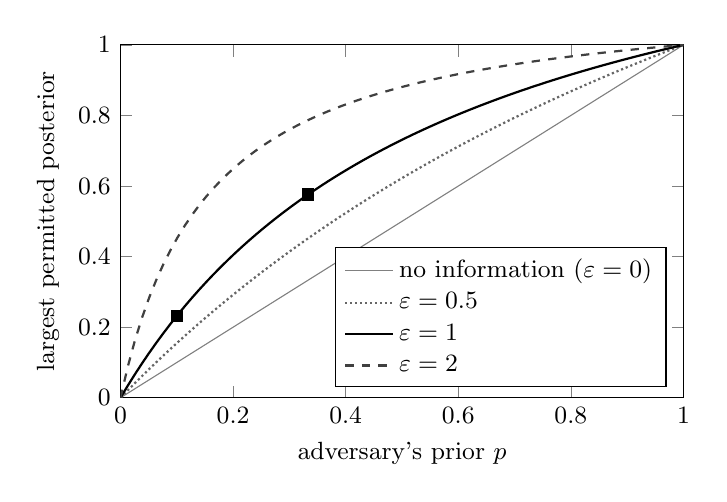
\begin{tikzpicture}
\begin{axis}[width=0.72\textwidth,height=0.5\textwidth,
  xmin=0,xmax=1,ymin=0,ymax=1,
  xlabel={adversary's prior $p$},ylabel={largest permitted posterior},
  legend pos=south east,legend cell align=left,
  tick label style={font=\small},label style={font=\small},legend style={font=\small}]
\addplot[domain=0:1,samples=2,thin,gray] {x};
\addlegendentry{no information ($\varepsilon=0$)}
\addplot[domain=0:1,samples=80,densely dotted,thick,black!60] {exp(0.5)*x/(exp(0.5)*x+1-x)};
\addlegendentry{$\varepsilon=0.5$}
\addplot[domain=0:1,samples=80,solid,thick,black] {exp(1)*x/(exp(1)*x+1-x)};
\addlegendentry{$\varepsilon=1$}
\addplot[domain=0:1,samples=80,dashed,thick,black!75] {exp(2)*x/(exp(2)*x+1-x)};
\addlegendentry{$\varepsilon=2$}
\addplot[only marks,mark=square*,mark size=2pt,black] coordinates {(0.1,0.232) (0.3333,0.576)};
\end{axis}
\end{tikzpicture}
\caption{The largest posterior an $\varepsilon$-differentially private release
permits, against the adversary's prior, from \eqref{c10:eq-post}. The curves are
told apart by line style as well as shade. The two squares mark the cases in the
text: a prior of 0.1 rises to at most 0.232, and a prior of one third to at most
0.576, at $\varepsilon = 1$.}
\label{c10:fig-post}
\end{figure}
% source for marked points: artifacts-paper/results.json, formal_privacy.posterior_bounds

The pipeline tabulates the bound for five values of $\varepsilon$ and three
priors. Take an adversary whose side information has narrowed the target to ten
candidates, so that its prior on each is 0.1. The guarantee permits a posterior
of 0.155 at $\varepsilon = 0.5$, 0.232 at $\varepsilon = 1$, 0.451 at
$\varepsilon = 2$ and 0.943 at $\varepsilon = 5$.
% source: artifacts-paper/results.json, formal_privacy.posterior_bounds (prior 0.1: 0.1548, 0.2320, 0.4509, 0.9428); paper/bis_ifc_full.tex lines 1303-1306
With a prior of one third, $\varepsilon = 1$ permits 0.576. With a prior of one in
a hundred, which is what an adversary holds if it knows only that the target lives
in a district of a hundred sampled people, $\varepsilon = 1$ permits 0.027 and
$\varepsilon = 5$ permits 0.600.
% source: artifacts-paper/results.json, formal_privacy.posterior_bounds (prior 0.01: epsilon 1 -> 0.0267, epsilon 5 -> 0.5999)

The misconception therefore confuses a multiplier with a level. An institution
that adopts $\varepsilon = 1$ has not chosen a tolerance. It has chosen a factor
of $e^\varepsilon$ on the odds of whatever prior an adversary brings, and the
re-identification risk it has implicitly accepted depends on what the adversary
knew before the release. The parameter cannot carry that information, because the
definition is built to hold for every prior at once. That is its strength as a
guarantee and the reason it cannot be read as a risk figure.

The last sentence of Proposition~\ref{c10:prop-post} deserves attention, because
most deployed mechanisms have $\delta > 0$. With $\delta > 0$ the likelihood ratio
on a rare output set can be arbitrarily large, so a posterior bound of the form
\eqref{c10:eq-post} holds only for most outputs, with $\varepsilon$ inflated, and
fails on a set of outputs of small probability \citep{kasiviswanathan2014}. The
usual reading of $\delta$ as ``the probability that the guarantee fails'' is
loose, but it points in the right direction: a mechanism with $\delta > 0$ may,
with small probability, publish something that identifies a person outright. A
committee that signs off on $\delta$ should know what it is signing for, and
$\delta$ should be small against the reciprocal of the number of people the
release covers \citep{dwork2014}.

Naledi's first page to the chair said this in plain words. The parameter in the
proposal was a ceiling on how much any reader of the monthly counts could learn
about one loan from the counts themselves. It was not the chance that someone
would identify a loan. That chance depended on what the reader already knew, and
the Bank's own scenarios, written for its loan-level files, said who those readers
were likely to be.

\section{From beliefs to attacks: a ceiling for every attack at once}

The posterior bound speaks about beliefs. A release committee needs a statement
about attacks, because its tolerance is a bound on the probability that a declared
attack succeeds. The bridge is a second reading of \eqref{c10:eq-dp}, as a limit on
hypothesis tests \citep{wasserman2010,kairouz2017,dong2022,balle2020}. Any attack
is a decision made from the output, and its success is an event; the definition
bounds the probability of every event under one database by its probability under
the neighbour.

Fix a target $t$ whose record sits in a known position of the database, and let
an attack be any rule $g$ that takes the release and the adversary's auxiliary
information $Z_t$ and names a position. Write $x$ for the database with the
target's record and $x^{(t)}$ for the database in which that record is replaced
by another drawn from a reference distribution. The attack's success
probability is
\begin{equation}\label{c10:eq-R}
R = \Prob\{g(M(x), Z_t) = t\},
\end{equation}
and its baseline is
\begin{equation}\label{c10:eq-kappa}
\kappa = \Prob\{g(M(x^{(t)}), Z_t) = t\},
\end{equation}
the probability that the same rule names the same position when the record there
is not the target's. The baseline is what the adversary achieves from everything
except the target's own contribution to the release: its auxiliary information,
the other records, and luck.

\begin{proposition}[A ceiling for every attack]\label{c10:prop-ceiling}
Let $M$ satisfy \eqref{c10:eq-dp} under the replace-one relation, and let the
adversary's auxiliary information $Z_t$ be independent of the mechanism's
randomness. Then for every attack rule $g$,
\begin{equation}\label{c10:eq-ceiling}
R \le \min\bigl(1,\ e^{\varepsilon}\kappa + \delta\bigr).
\end{equation}
Consequently a tolerance $\tau$ is met by all attacks together whenever
$e^{\varepsilon}\kappa^\ast + \delta \le \tau$, where $\kappa^\ast$ is the largest
baseline success the institution admits over the attacks it is willing to
consider.
\end{proposition}

This is the inequality at which the two regimes meet, and it is worth reading
slowly. The privacy parameter supplies the multiplier $e^\varepsilon$ and the
additive slack $\delta$, and it does so for every rule $g$ at once, including
rules nobody at the Bank has thought of. What it does not supply is $\kappa$. The
baseline is a property of the adversary's knowledge and the rest of the data, and
an argument about it is exactly the kind of argument that scenario assessment
makes. A differentially private release therefore does not remove the need for a
declared adversary. It changes the question the scenario must answer, from ``how
often does this attack succeed?'' to ``how well could anyone do without the
target's own record?'', and it turns the answer into a ceiling that holds for
every attack.

The inequality also yields a test that a committee can run on the back of an
envelope. Hold the Bank's tolerance of 0.12 and set $\delta$ negligible. At
$\varepsilon = 1$ the ceiling meets the tolerance whenever the baseline is below
$0.12/e$, about 0.044; at $\varepsilon = 2$ the baseline must be below about
0.016.
% derived: tau = 0.12 (paper/generated/numbers.tex \runevaltolerance) divided by e^1 = 2.718 and e^2 = 7.389
A baseline of 0.044 is the success of a uniform guess among about 23 candidates.
% derived: 1/0.0441 = 22.7
If the Bank can argue that no plausible reader of its counts can narrow a loan down
below that many candidates without the loan's own contribution, the monthly
counts meet the tolerance against every attack. If it cannot, the guarantee is
still true, and it still says nothing the committee can use.

\citet{kifer2014} make the adversary's prior an explicit input to a privacy
definition in the Pufferfish framework, which is the formal counterpart of a
declared scenario, and \citet{kifer2011} show that no privacy definition can be
free of assumptions about the data-generating process if it is to bound what an
adversary learns about a person. These results give the ceiling its place. The
guarantee in \eqref{c10:eq-dp} compares two databases and needs no such
assumption. The moment one asks what an adversary believes about a person, which
is what \eqref{c10:eq-post} and \eqref{c10:eq-ceiling} do, an assumption enters:
in Proposition~\ref{c10:prop-post} that the other records have the same
distribution under both hypotheses, and in Proposition~\ref{c10:prop-ceiling} a
reference distribution for the replacement record that fixes $\kappa$.

\section{Noisy counts on the credit register}\label{c10:sec-counts}

The pipeline runs the supervision department's proposal on the synthetic credit
register of Chapter~\ref{ch:credit}, and the results show both readings of the
guarantee at work. The release publishes, for the first vintage, a noisy count of
live loans in each of 814 occupied cells of sector, region and size class, of which
10 hold a single loan.
% source: artifacts-paper/results.json, evaluation.policies[dp_counts_*].identification (cells 814, unique_cells 10)
The declared adversary attacks the cells, not the loans: it reads each noisy
count, computes the posterior that the true count is one against a prior built
from the distribution of cell sizes, and declares a cell to hold a single,
identifiable loan when that posterior reaches one half. Its success is a correct
declaration.

At $\varepsilon = 1$ for one month the adversary never acts: no cell reaches the
threshold, and the exact one-sided 95 per cent bound on its success over the 814
cells is 0.0037. At $\varepsilon = 5$ it acts on 11 cells and is right on 10 of
them, so it finds every singleton the release contains, with a precision of 0.909.
% source: artifacts-paper/results.json, evaluation.policies dp_counts_1.identification (decisions 0, success_upper 0.00367) and dp_counts_5.identification (decisions 11, true_positive 10, precision 0.909, recall 1.0); paper/generated/numbers.tex \runevalcountsprecision, \runevalcountsrecall
The contrast follows the curves of Figure~\ref{c10:fig-post}. The adversary's
prior that a cell is a singleton is small, about 10 in 814, and at
$\varepsilon = 1$ a reading of the count cannot move it to one half. At
$\varepsilon = 5$ the noise has scale 0.2, a reading near one leaves little doubt,
and the prior no longer protects.

Over six monthly vintages the programme spends six times the monthly parameter
under basic composition, 6 at $\varepsilon = 1$ and 30 at $\varepsilon = 5$. The
pooled adversary, which multiplies the likelihoods of all six readings, acts on 7
cells at $\varepsilon = 1$ and is right on 4.
% source: artifacts-paper/results.json, evaluation.policies dp_counts_1.identification_pooled (epsilon_total 6, decisions 7, true_positive 4) and dp_counts_5.identification_pooled (epsilon_total 30)
The accounting predicted that the programme would leak more than one month, and
it did.

One result in the run cuts the other way and is reported because it is
instructive. At $\varepsilon = 5$ the pooled adversary does worse than the
single-month one: it acts on 6 cells and is right on 4, against 10 of 11 from one
month.
% source: artifacts-paper/results.json, evaluation.policies dp_counts_5.identification_pooled (decisions 6, true_positive 4)
The reason is in the attack, not the mechanism. The pooled adversary assumes that a
cell's count is the same in every vintage, while in the register loans leave and
arrive, so its likelihood is wrong and averaging over six readings blurs a count
that one reading had nearly pinned. A scenario assessment measures the attack it
was given. The ceiling of Proposition~\ref{c10:prop-ceiling} holds for the better
attack nobody ran, which is why the two figures must not be read against each
other on one scale.

The cost side is just as plain. On the utility scale used for the credit products,
where the unprotected loan-level file scores 0 and the 5-anonymous loan-level file
scores $-0.050$, the noisy counts score $-0.40$ at $\varepsilon = 1$ and $-0.36$ at
$\varepsilon = 5$.
% source: artifacts-paper/results.json, evaluation.policies (dp_counts_1 utility -0.40, dp_counts_5 utility -0.36); paper/generated/table_evaluation.tex (k=5 utility -0.050)
A product with no microdata cannot serve the lender-level and concentration
analyses the register is collected for, whatever its noise. The comparison is not
like for like, since the targets of the counts attack are cells and those of the
loan-level attacks are loans, and Chapter~\ref{ch:credit} keeps them out of its
comparison of policies for that reason.

The chair read the results with a question of her own. If the monthly counts at
$\varepsilon = 1$ defeat the declared attack, why could the Bank not simply say so
and stop? Naledi's answer was that the declared attack was one reader. The
guarantee covered all readers, but only through the baseline, and the Bank had not
yet written down what a lender that knows its own borrowers could achieve without
the counts. That was the next piece of work.

\section{Accounting across a programme}

Chapter~\ref{ch:programmes} proved that no function of per-release risks can bound
the risk of an adversary who pools the releases (Proposition~\ref{prop:nopool}).
Formal privacy is the one framework in which the opposite holds: guarantees add up
across releases with no assumption about how the releases depend on one another.

\begin{proposition}[Basic composition]\label{c10:prop-comp}
Let mechanisms $M_1,\dots,M_m$ act on one database, where $M_i$ may be
chosen in the light of the outputs of $M_1,\dots,M_{i-1}$, and suppose each $M_i$
is $(\varepsilon_i,\delta_i)$-differentially private under the same neighbouring
relation whatever those earlier outputs were. Then the joint output is
$(\sum_i \varepsilon_i, \sum_i \delta_i)$-differentially private. Combined with
Proposition~\ref{c10:prop-ceiling}, any attack that uses all $m$ outputs succeeds
with probability at most
\begin{equation}\label{c10:eq-progceiling}
R_{\mathrm{pool}} \le \min\Bigl(1,\ e^{\sum_i \varepsilon_i}\,\kappa_{\mathrm{pool}} + \sum_i \delta_i\Bigr),
\end{equation}
where $\kappa_{\mathrm{pool}}$ is the baseline of the pooled attack.
\end{proposition}

Inequality \eqref{c10:eq-progceiling} is the composition theorem that scenario
assessment lacks, and its price is visible at once. The exponent adds, so the
multiplier grows geometrically. Six months at $\varepsilon = 1$ give a multiplier
of $e^6$, about 403, and the Bank's tolerance of 0.12 is then met only if the
pooled baseline is below about 0.0003.
% derived: e^6 = 403.4; 0.12 / 403.4 = 2.97e-4; tolerance from paper/generated/numbers.tex \runevaltolerance
The ceiling is valid, and for most practical baselines it is vacuous. That is not
a defect of the theorem. The basic rule is loose, and much of the later work on
formal privacy has gone into tightening it.

Advanced composition \citep{dwork2010} shows that $m$ mechanisms each with
parameter $\varepsilon$ compose, at the cost of a small extra $\delta$, to a total
that grows like $\sqrt{m}\,\varepsilon$ for small $\varepsilon$, not like
$m\varepsilon$. \citet{kairouz2017} give the exact composition of
$(\varepsilon,\delta)$ guarantees, read as limits on tests. Rényi differential
privacy \citep{mironov2017} and concentrated differential privacy
\citep{bun2016} track a whole curve of divergences between the output
distributions on neighbours, which adds exactly across mechanisms and converts to
an $(\varepsilon,\delta)$ statement only at the end; Gaussian differential privacy
\citep{dong2022} does the same with a single parameter for mechanisms that add
Gaussian noise. These accountants are what a programme should run. They are not
different definitions of privacy, and each converts back into
\eqref{c10:eq-dp}, so Proposition~\ref{c10:prop-ceiling} applies to whatever they
report.

Two further devices address a problem that is particular to programmes. The
parameters of later releases are often chosen after earlier ones are out: a user
asks for one more table, a department wants a finer breakdown. A privacy filter is
a rule that, given a total budget fixed in advance, allows each new release only if
the running account stays inside the budget, and halts the programme otherwise;
the composition guarantee then holds for the total even though the parameters were
chosen as the programme ran. A privacy odometer goes one step further and reports,
at every point, a running bound on the loss so far that is valid whenever it is
read. The two play the role for privacy accounting that the anytime-valid bounds of
Chapter~\ref{ch:monitoring} play for attack simulation: they keep a guarantee true
when the analyst looks at the account and decides what to do next. A committee
that lets parameters be set release by release needs one of them in its record,
because basic or advanced composition stated for fixed parameters does not cover
choices made in the light of earlier outputs.

The contrast with Chapter~\ref{ch:programmes} can now be stated without
overstatement. For scenario assessment the per-release figures say nothing about
the pooled attack, and the institution must simulate the joint attack directly.
For formal privacy the per-release parameters bound the joint guarantee, and the
institution must still argue for a pooled baseline before the guarantee becomes a
risk figure. In both regimes the programme needs a horizon. Without one, the
pooled risk in the first regime and the accumulated budget in the second have no
fixed meaning.

Tomás's request made this concrete for the Bank. He asked for the monthly counts
for the full six months, and also for a finer table by lender. Under the Bank's
current practice the second table would have been assessed on its own. Under a
formal accountant it had to come out of the same budget as the first, and Naledi's
note to the chair said the Bank could release the second table only by spending
budget that the first had already used.

\section{What the guarantee does not name}\label{c10:sec-unnamed}

A differential privacy guarantee is precise about one thing, the effect of one
record, and silent about several others that a release committee must still
govern.

The first is the unit. The guarantee protects whatever the neighbouring relation
changes. If the mechanism treats a loan as the record, a firm with several loans is
protected only as a group, and the group guarantee degrades with its size.

\begin{proposition}[Groups]\label{c10:prop-group}
If $M$ is $\varepsilon$-differentially private, then for databases $x$ and $x''$
that differ in the records of $g$ individuals,
$\Prob\{M(x) \in E\} \le e^{g\varepsilon}\,\Prob\{M(x'') \in E\}$ for every
measurable $E$.
\end{proposition}

In the synthetic credit register a borrower holds between one and four lending
relationships.
% source: paper/bis_ifc_full.tex, Appendix "Simulation details", paragraph "Credit register" (between one and four lending relationships)
A loan-level guarantee at $\varepsilon = 1$ is therefore, for the largest
borrowers, a borrower-level guarantee at $\varepsilon = 4$, and by
Figure~\ref{c10:fig-post} a prior of 0.1 can then rise much further. The
largest borrowers are also the ones most easily singled out by other means, so the
weakest guarantee falls on the most exposed firms. A committee should state the
unit of protection in its record and choose it to match the party the law
protects, which for a credit register is usually the borrower.

The second is inference from the population. Differential privacy bounds what the
release reveals about a person beyond what it would reveal if their record were
absent. If the release shows that firms in a sector are mostly in arrears, a reader
can infer that a given firm in that sector is probably in arrears, whether or not
its loan was in the data \citep{dwork2014}. That inference is the purpose of
statistics, and no mechanism that keeps the release useful can prevent it. It is
also a form of attribute disclosure that a committee may care about for small
groups, and the guarantee does not address it.

The third is dependence between records. Proposition~\ref{c10:prop-post} assumes
that the other records have the same distribution whether or not $H$ holds. In a
register of linked firms, or of a borrower's several loans, removing one record
does not remove the information the others carry about it, and the posterior
reading can fail even though \eqref{c10:eq-dp} holds \citep{kifer2011}.

The fourth is the legal notion of identification. \citet{cohen2020} study how the
data protection notion of singling out can be stated formally and how
differential privacy relates to it. Their analysis is a reminder that a
guarantee about output distributions has to be connected, by an argument, to the
words a regulator uses, and that the connection is not automatic.

\section{Hazards in implementation}

A guarantee is a property of a mechanism as specified. A deployed mechanism can
fail to have it for reasons that have nothing to do with the mathematics, and a
committee that relies on the guarantee should ask about each of them.

The sensitivity may be stated for the wrong relation or the wrong unit. The noise
scale $1/\varepsilon$ used for counts gives $\varepsilon$ under add-or-remove for a
single loan. Under replace-one, a loan that moves from one cell to another changes
two counts, and the same noise gives $2\varepsilon$; for a borrower with four loans
the factor is four. Each of these is a correct guarantee for some statement, and a
record that names the parameter without the relation and the unit has not said
which.

The noise may not be the noise in the proof. A Laplace or Gaussian draw computed in
floating-point arithmetic is not exactly the continuous distribution the proof
assumes, and naive sampling code can leave patterns in the low-order digits of the
output that reveal the value underneath. Implementations designed for formal
privacy sample from discrete distributions with exact arithmetic for this reason.
Rounding or clamping after noise is added is safe, since anything computed from
the output alone keeps the guarantee; clamping the data before the noise, to bound
sensitivity, must be part of the stated mechanism.

The budget may be spent where nobody counts it. Choosing $\varepsilon$, the
query, the cells or the release date after looking at the confidential data is
itself a use of the data, and so is a data-dependent decision to suppress or
republish. Releasing a noisy figure, discarding it and drawing again because the
first looked odd spends the budget twice. Reusing one noise draw across months,
in the other direction, breaks the independence that the per-month accounting
assumes; the pipeline's monthly counts draw fresh noise each vintage for this
reason.
% source: src/privacy_risk/evaluation.py, counts_attack docstring ("each vintage publishes its own noisy counts with a fresh draw of noise")

The code may have errors that no review catches. Empirical auditing turns the
ceiling of Proposition~\ref{c10:prop-ceiling} around: an attack whose success
exceeds $e^\varepsilon\kappa + \delta$ for a measurable baseline is evidence that
the mechanism does not have the claimed parameter. \citet{jagielski2020} use
attacks of this kind to put lower bounds on the privacy loss of private training
of machine learning models, and \citet{steinke2023} show how to do so with a single
run of the training procedure. The same logic applies to a noisy-count release,
and the attack simulation machinery of Chapter~\ref{ch:estimate} is what it needs.
A falsification test of this kind belongs among those of Part~VI.

Finally, some products carry the vocabulary without the guarantee. Synthetic data
generated by a model fitted without a privacy mechanism are not protected by any
parameter, and \citet{stadler2022} show that such data can leak the records they
were trained on. A release described as private should state a mechanism, a
relation, a unit and an accountant, and if it cannot state all four it should be
assessed as a scenario release.

\section{Two regimes in one record}

The chapter asked what a privacy-loss parameter commits an institution to, in the
units a release decision uses. The answer is now available.

Adopting $\varepsilon = 1$ commits the institution to a release whose output
changes by at most a factor of $e$ when one record changes. In the units of a
release decision this is a commitment of two kinds. Against beliefs, it multiplies
the odds an adversary already holds by at most $e$: a prior of 0.1 can become
0.232, and a prior of one third can become 0.576. Against attacks, it caps the
success of every attack at $e^\varepsilon\kappa + \delta$, where $\kappa$ is what
the attack could achieve without the target's own record. Neither statement is a
low re-identification risk until someone argues that the adversary's prior, or the
baseline, is small. That argument is a declared scenario, and the institution must
write it down in exactly the form earlier chapters require.

So the two regimes answer different questions and both belong in the record.
Scenario assessment is adversary-specific: it says what a named adversary achieves
against this release, the question a governance committee, a data protection
authority and an affected person all ask. Formal privacy is adversary-agnostic: it
says how far any observer's beliefs can move because one record was included, and
it is the only device that composes across a programme without an assumption about
how the releases relate. An institution that wants both should hold both, running
a formal accountant for the programme budget and a scenario assessment for each
release decision, reporting them separately with their assumptions. They meet at
\eqref{c10:eq-ceiling}, and for a differentially private release the scenario
assessment is then needed only to argue for $\kappa$.

Grace read the decision record for the monthly counts some months later. It named
$\varepsilon$, the add-or-remove relation, the loan as the unit, the accountant and
the six-month horizon. Beside them it named the adversary the Bank had in mind, the
baseline it had argued for that adversary, and the ceiling that followed. She had
no question to ask about the parameter. Her one note concerned the unit, and asked
why the record protected loans when the law protected borrowers.

\begin{inpractice}[In practice: a release that carries a privacy parameter]
Record four things beside $\varepsilon$ and $\delta$: the neighbouring relation,
the unit of protection, the accountant used across the programme, and the horizon
over which the budget is spent. Then translate the parameter into the Bank's own
units. For each declared adversary, state its prior or its baseline success
$\kappa$ without the target's record, and report the posterior bound
\eqref{c10:eq-post} or the ceiling $\min(1, e^\varepsilon\kappa + \delta)$ beside
the tolerance. If the ceiling exceeds the tolerance, the guarantee does not support
the release, however small $\varepsilon$ looks. If parameters may be chosen as the
programme runs, use a filter or an odometer, and count every look at the
confidential data, including decisions to redraw or withdraw, against the budget.

\sloppy\smallskip\noindent\textit{In the software.} The posterior bound
\eqref{c10:eq-post} and basic composition are in \texttt{privacy\_risk.dp}
(\texttt{posterior\_bound}, \texttt{posterior\_bound\_table} and
\texttt{basic\_composition}); the table quoted in this chapter is produced by
\texttt{experiments.formal\_privacy}. The noisy-count release and its single-month
and pooled attacks are in \texttt{privacy\_risk.evaluation}
(\texttt{counts\_attack}). The package does not yet compute the ceiling
\eqref{c10:eq-ceiling} or any accountant tighter than the basic one; both are
short additions. The bound itself is a few lines:
\begin{lstlisting}
def posterior_bound(epsilon: float, prior: float) -> float:
    """Largest posterior an (epsilon, 0)-differentially private release permits.

    With delta > 0 no uniform posterior bound exists, so this function covers the
    pure case only.
    """
    if epsilon < 0:
        raise ValueError("epsilon must be nonnegative")
    if not 0 <= prior <= 1:
        raise ValueError("the prior must be a probability")
    factor = math.exp(epsilon)
    return float(factor * prior / (factor * prior + (1 - prior)))
\end{lstlisting}
\end{inpractice}

\section{Proofs}

\begin{proof}[Proof of Proposition~\ref{c10:prop-post}]
Write $W$ for the records other than the individual's, with the same law under
$H$ and under its negation, and let $r$ and $r'$ be the individual's record under
$H$ and under its negation (each may itself be random, independent of $W$). For
each value $w$ of the other records, the databases $(w, r)$ and $(w, r')$ are
neighbours under the replace-one relation, so by \eqref{c10:eq-dp} with
$\delta = 0$, $\Prob\{M(w,r) \in E\} \le e^\varepsilon \Prob\{M(w,r') \in E\}$.
Integrating both sides over the common law of $W$ and over the laws of $r$ and
$r'$ gives
$\Prob(M \in E \mid H) \le e^\varepsilon \Prob(M \in E \mid \neg H)$. Bayes' rule
in odds form then gives
\[
\frac{\Prob(H \mid M \in E)}{1 - \Prob(H \mid M \in E)}
= \frac{p}{1-p}\cdot\frac{\Prob(M \in E \mid H)}{\Prob(M \in E \mid \neg H)}
\le \frac{p}{1-p}\,e^{\varepsilon},
\]
and since $u \mapsto u/(1-u)$ is increasing on $[0,1)$, solving for the posterior
gives \eqref{c10:eq-post}. If $\Prob(M \in E \mid \neg H) = 0$ then
$\Prob(M \in E \mid H) = 0$ as well and $E$ has probability zero, which is
excluded.

For $\delta > 0$ the same steps give
\[
\frac{\Prob(H \mid M \in E)}{1 - \Prob(H \mid M \in E)}
\le \frac{p}{1-p}\Bigl(e^{\varepsilon} + \frac{\delta}{\Prob(M \in E \mid \neg H)}\Bigr),
\]
and the last term is unbounded as $\Prob(M \in E \mid \neg H) \to 0$. To see that
no uniform bound survives, take a mechanism that with probability $\delta$
publishes the individual's record and otherwise publishes nothing. It satisfies
\eqref{c10:eq-dp} with $\varepsilon = 0$ and this $\delta$, and on the output set
in which the record is published under $H$ the posterior on $H$ is one whatever the
prior.
\end{proof}

\begin{proof}[Proof of Proposition~\ref{c10:prop-ceiling}]
Fix a value $z$ of the auxiliary information and a value of the database apart from
the target's position. The event $E_z = \{y : g(y, z) = t\}$ is a measurable set
of outputs, and the databases $x$ and $x^{(t)}$ differ only in the record at the
target's position, so they are neighbours. By \eqref{c10:eq-dp},
\[
\Prob\{M(x) \in E_z\} \le e^{\varepsilon}\Prob\{M(x^{(t)}) \in E_z\} + \delta .
\]
Because $Z_t$ is independent of the mechanism's randomness, integrating both sides
over the law of $Z_t$, over the other records and over the reference law of the
replacement record leaves the inequality intact and gives
$R \le e^{\varepsilon}\kappa + \delta$ by \eqref{c10:eq-R} and
\eqref{c10:eq-kappa}. Since $R$ is a probability, $R \le 1$, which gives
\eqref{c10:eq-ceiling}. If $e^{\varepsilon}\kappa^\ast + \delta \le \tau$ and every
admitted attack has baseline at most $\kappa^\ast$, every admitted attack has
$R \le \tau$.
\end{proof}

\begin{proof}[Proof of Proposition~\ref{c10:prop-comp}]
We prove the case $\delta_i = 0$ for all $i$ with outputs in countable sets, which
carries the idea; the general case, including $\delta_i > 0$ and adaptive choice,
is in \citet[ch.~3]{dwork2014}. Let $x \sim x'$ and let
$y = (y_1,\dots,y_m)$ be a joint output. By the chain rule,
\[
\Prob\{(M_1,\dots,M_m)(x) = y\}
= \prod_{i=1}^m \Prob\{M_i(x) = y_i \mid y_1,\dots,y_{i-1}\},
\]
where the $i$th factor is the probability that the mechanism chosen after
$y_1,\dots,y_{i-1}$ outputs $y_i$ on $x$. Each factor is at most $e^{\varepsilon_i}$
times the corresponding factor for $x'$, by the hypothesis on $M_i$ applied to the
singleton $\{y_i\}$. Multiplying, the joint probability under $x$ is at most
$e^{\sum_i \varepsilon_i}$ times that under $x'$, and summing over the outputs in
any set $E$ gives \eqref{c10:eq-dp} for the joint mechanism with
$\varepsilon = \sum_i\varepsilon_i$ and $\delta = 0$. The bound
\eqref{c10:eq-progceiling} follows by applying Proposition~\ref{c10:prop-ceiling}
to the joint mechanism, with the pooled attack as the rule $g$.
\end{proof}

\begin{proof}[Proof of Proposition~\ref{c10:prop-group}]
Let $x = x_0, x_1, \dots, x_g = x''$ be a chain of databases in which each
consecutive pair differs in the record of one of the $g$ individuals, so that
consecutive members are neighbours. Applying \eqref{c10:eq-dp} with $\delta = 0$
along the chain gives
$\Prob\{M(x_0) \in E\} \le e^{\varepsilon}\Prob\{M(x_1) \in E\} \le \dots
\le e^{g\varepsilon}\Prob\{M(x_g) \in E\}$.
\end{proof}
